\section{Paper Reading: DANet (TODO)}


\begin{frame}{Dual Attention Network for Scene Segmentation}
    \begin{itemize}
        \item \textbf{Title:} Dual Attention Network for Scene Segmentation
        \item \textbf{Author:} Jun Fu, Jing Liu, Haijie Tian, Yong Li, Yongjun Bao, Zhiwei Fang, Hanqing Lu
        \item \textbf{Comments:} Accepted by CVPR2019
        % \item \textbf{Contribution:} \textbf{Propose} an end-to-end Correlation-guided Discriminative Learning (CDL) model to fully mine and exploit the discriminative potentials of correlations for WFGIC globally and locally. 
        % \footnote{提出了一个端到端相关性引导判别学习(CDL)模型,以充分挖掘和利用相关性在全局和局部的鉴别潜力。}
        % \item 开源代码:无
        
        \item \textbf{arxiv:}https://arxiv.org/pdf/1809.02983.pdf
    \end{itemize}
\end{frame}


\begin{frame}{Non-local}
    \textbf{Non-local}
    \begin{equation}
        y_i=\frac{1}{C(x)}\sum_{\forall j}f(x_i,x_j)g(x_j)
    \end{equation}
    $C(x)$是归一化系数,$f(x_i,x_j)$用来计算输入信号在$x_j$位置与$x_i$的相似性/相关性,并且对$g(x_j)$进行加权,$g(x_j)$计算输入信号在$j$位置的特征值。
    \begin{itemize}
        \item \textbf{Gaussian.} $f(x_i,x_j)=e^{x_i^T x_j}$, $C(x)=\sum_{\forall j}f(x_i,x_j)$
        \item \textbf{Embedded Gaussian.} $f(x_i,x_j)=e^{\theta(x_i)^T \Phi(x_j)}$, $C(x)=\sum_{\forall j}f(x_i,x_j)$
        \item \textbf{Dot product.} $f(x_i,x_j)=\theta(x_i)^T \Phi(x_j)$, $C(x)=N$
        \item \textbf{Concatenation.} $f(x_i,x_j)=ReLU(w_f^T [\theta(x_i),\Phi(x_j)])$, $C(x)=N$
    \end{itemize}
\end{frame}

\begin{frame}{DANet}
    \begin{figure}
        \centering
        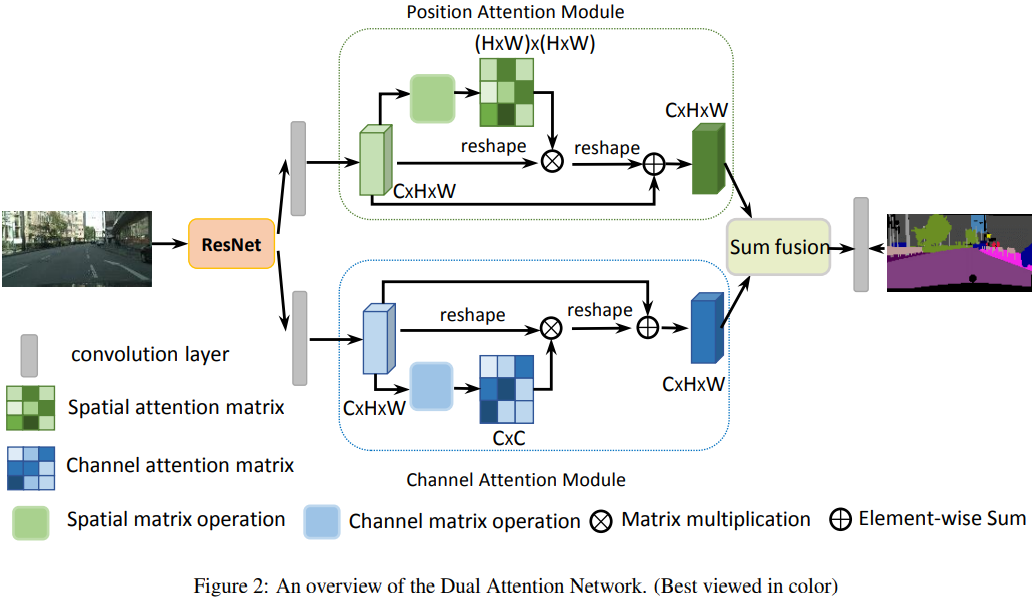
\includegraphics[width=0.8\textwidth]{docs/paperReading/danet/danet.png}
    \end{figure}
\end{frame}

\begin{frame}{DANet:PAM and CAM}
    \begin{figure}
        \centering
        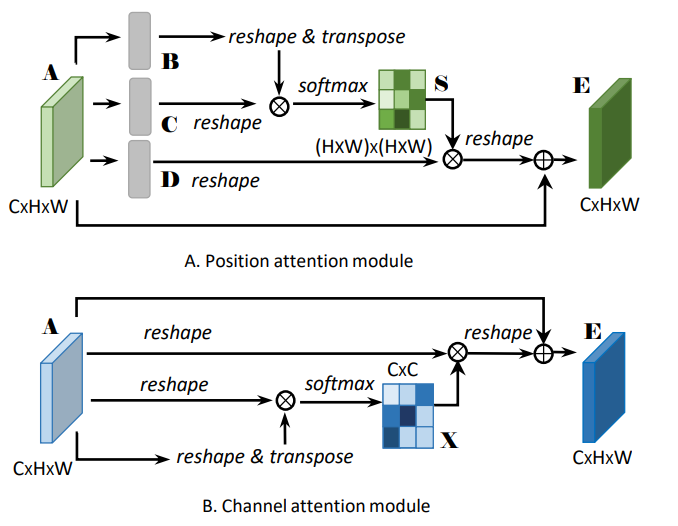
\includegraphics[width=0.45\textwidth]{docs/paperReading/danet/pam_cam.png}
    \end{figure}

    \begin{itemize}
        \item \textbf{PAM} Position attention module
        \item \textbf{CAM} Channel attention module
    \end{itemize}
\end{frame}


% \begin{frame}{experiment}
%     \begin{multicols}{2}
%         \begin{figure}
%             \centering
%             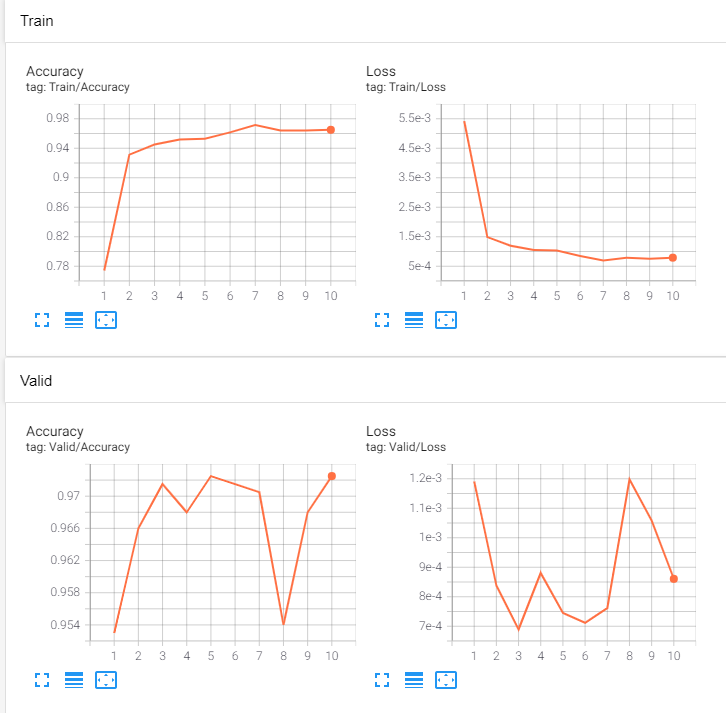
\includegraphics[width=0.4\textwidth]{docs/paperReading/danet/lr_0001.png}
%             \caption{lr=0.0001}
%         \end{figure} 
%         \begin{figure}
%             \centering
%             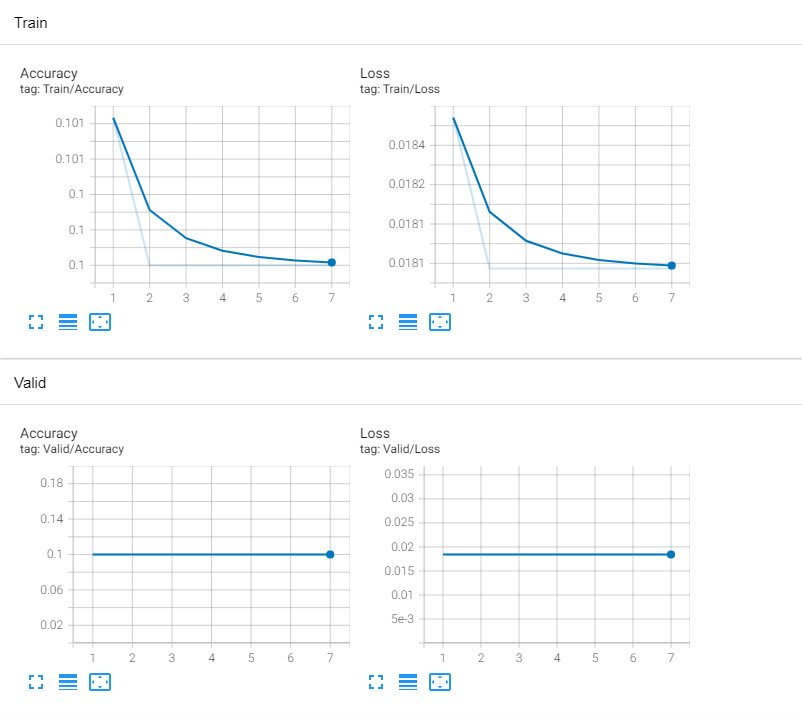
\includegraphics[width=0.4\textwidth]{docs/paperReading/danet/lr_001.png}
%             \caption{lr=0.001}
%         \end{figure} 
%     \end{multicols}
% \end{frame}
